\section{Applying MUA to vault and attempting deletion}

\subsection{Creating a resource guard}\label{MUA}
In order to enable Multi User Authentication, a resource guard must be created in a different subscription or directory than the backup vault, but they must be in the same region.

In a different Azure subscription than the one containing the Revocery Services vault, the security admin creates a resource guard. This can be done with the following command in powershell: 

\begin{minted}[breaklines=true,breakanywhere=true]{powershell}
New-AzResource -Location "North Europe" -ResourceName "BackupRG" -ResourceType "Microsoft.DataProtection/resourceGuards" -ResourceGroupName "bProject"

which gives the following output:

Name              : BackupRG
ResourceId        : /subscriptions/c29c75c2-44ed-4c7e-a49f-12ebe97637dd/resourceGroups/bProject/providers/Microsoft.DataProtection/resourceGuards/BackupRG
ResourceName      : BackupRG
ResourceType      : Microsoft.DataProtection/resourceGuards
ResourceGroupName : bProject
Location          : northeurope
SubscriptionId    : c29c75c2-44ed-4c7e-a49f-12ebe97637dd
Properties        : @{provisioningState=Succeeded; resourceGuardOperations=System.Object[]; vaultCriticalOperationExclusionList=System.Object[]; 
                    allowAutoApprovals=True}
\end{minted}

By default the resource guard has all protected operations enabled by default, but the security admin can choose to disable some protections. \textit{Disable soft delete} and \textit{Remove MUA protection} cannot be disabled. See the following image for how this looks in the Azure GUI. 

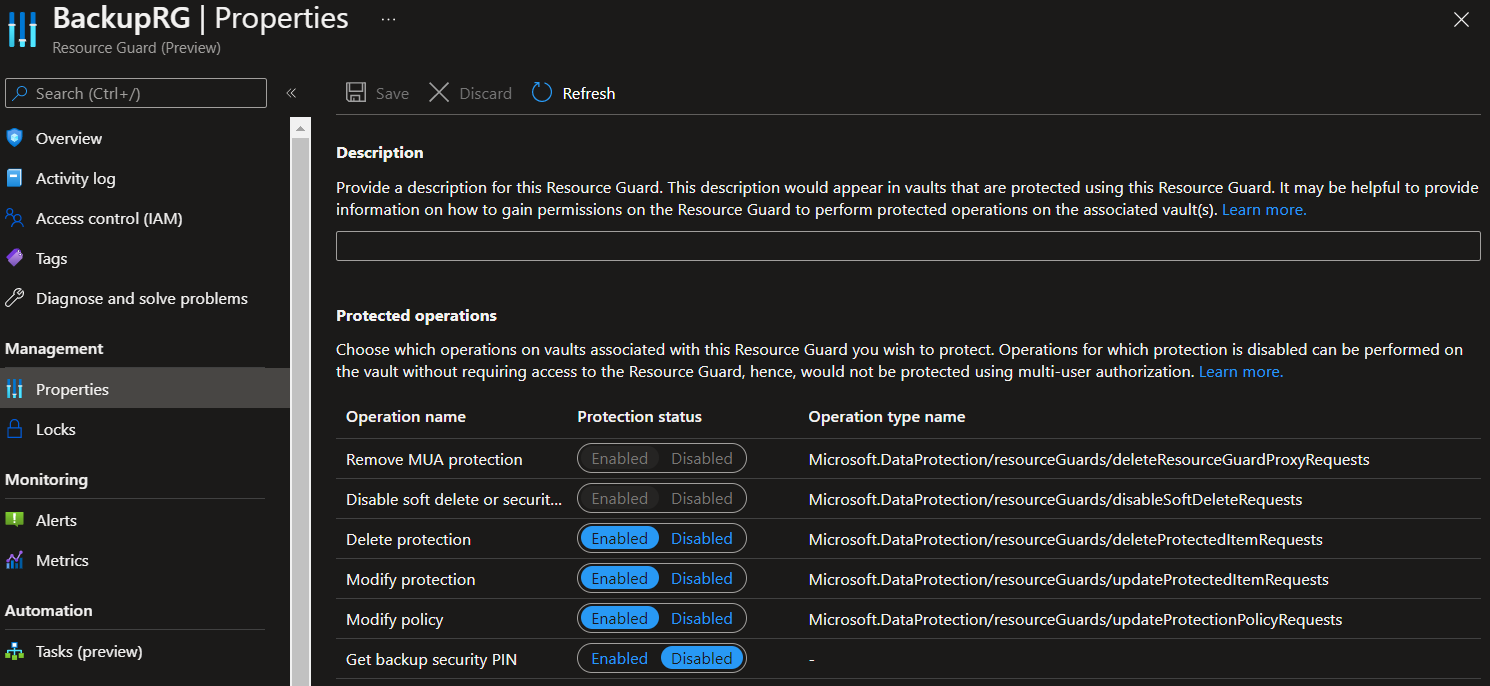
\includegraphics[width=.9\linewidth]{figures/RG-properties.PNG}
%Define properties for width etc.

\subsection{Assigning reader role to backup admin}
The next step is to assign the reader role on the Resource Guard to the backup administrator account. In the GUI we can do this through the Access control(IAM)-blads. In the following images we add the reader role on the Resource guard to the user that acts as the backup admin in this example.

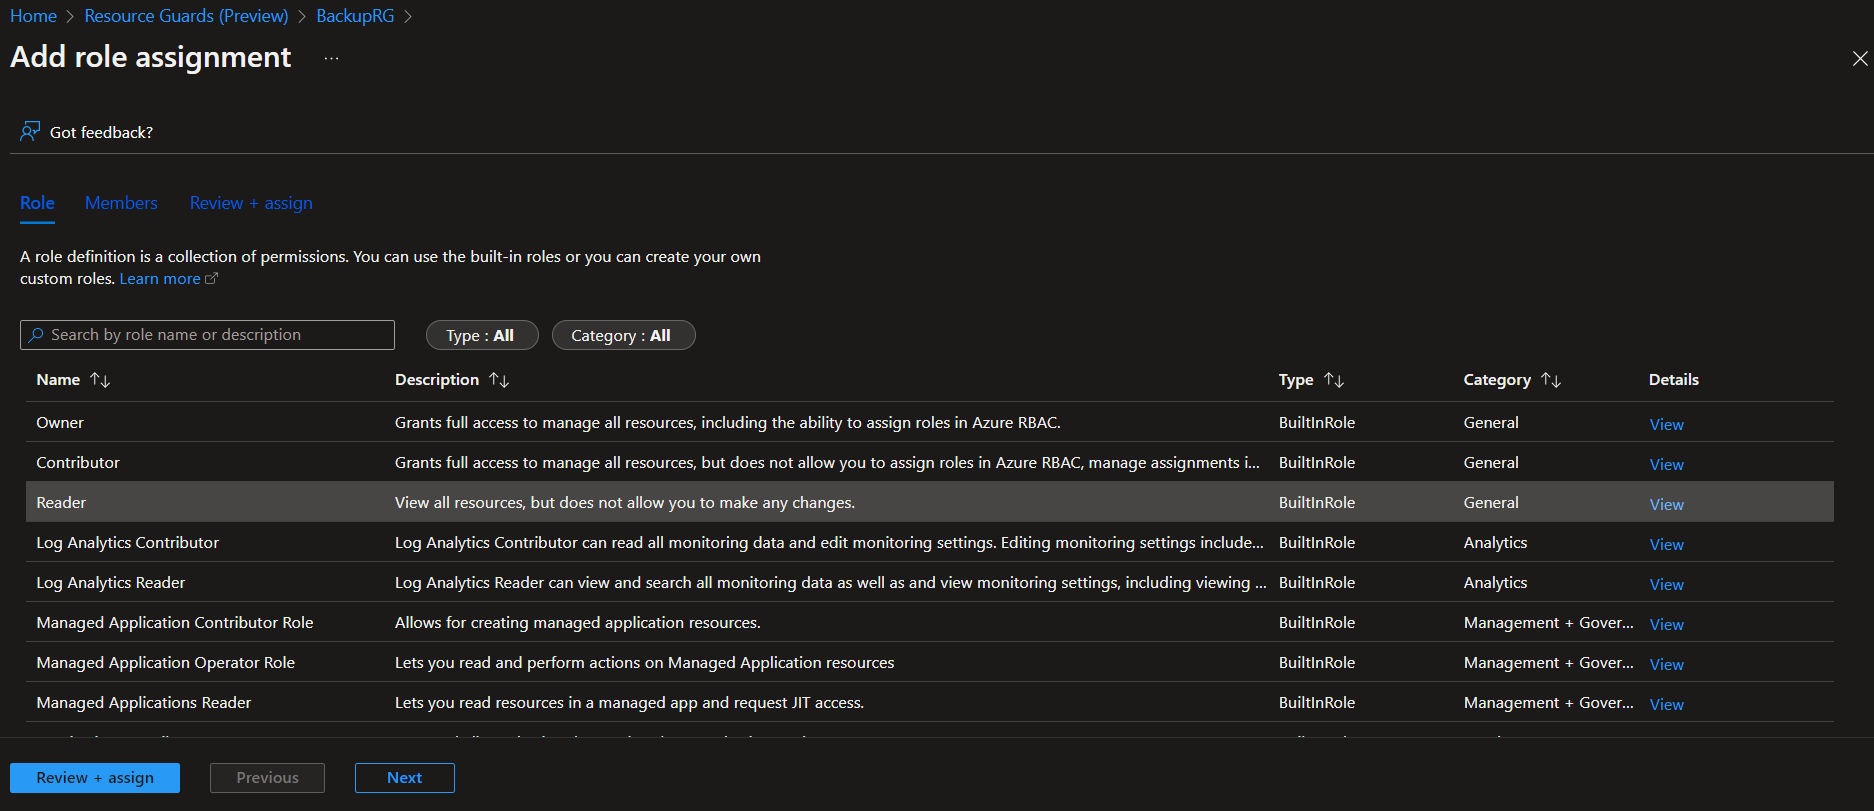
\includegraphics[width=.9\linewidth]{figures/RG-roles.PNG}

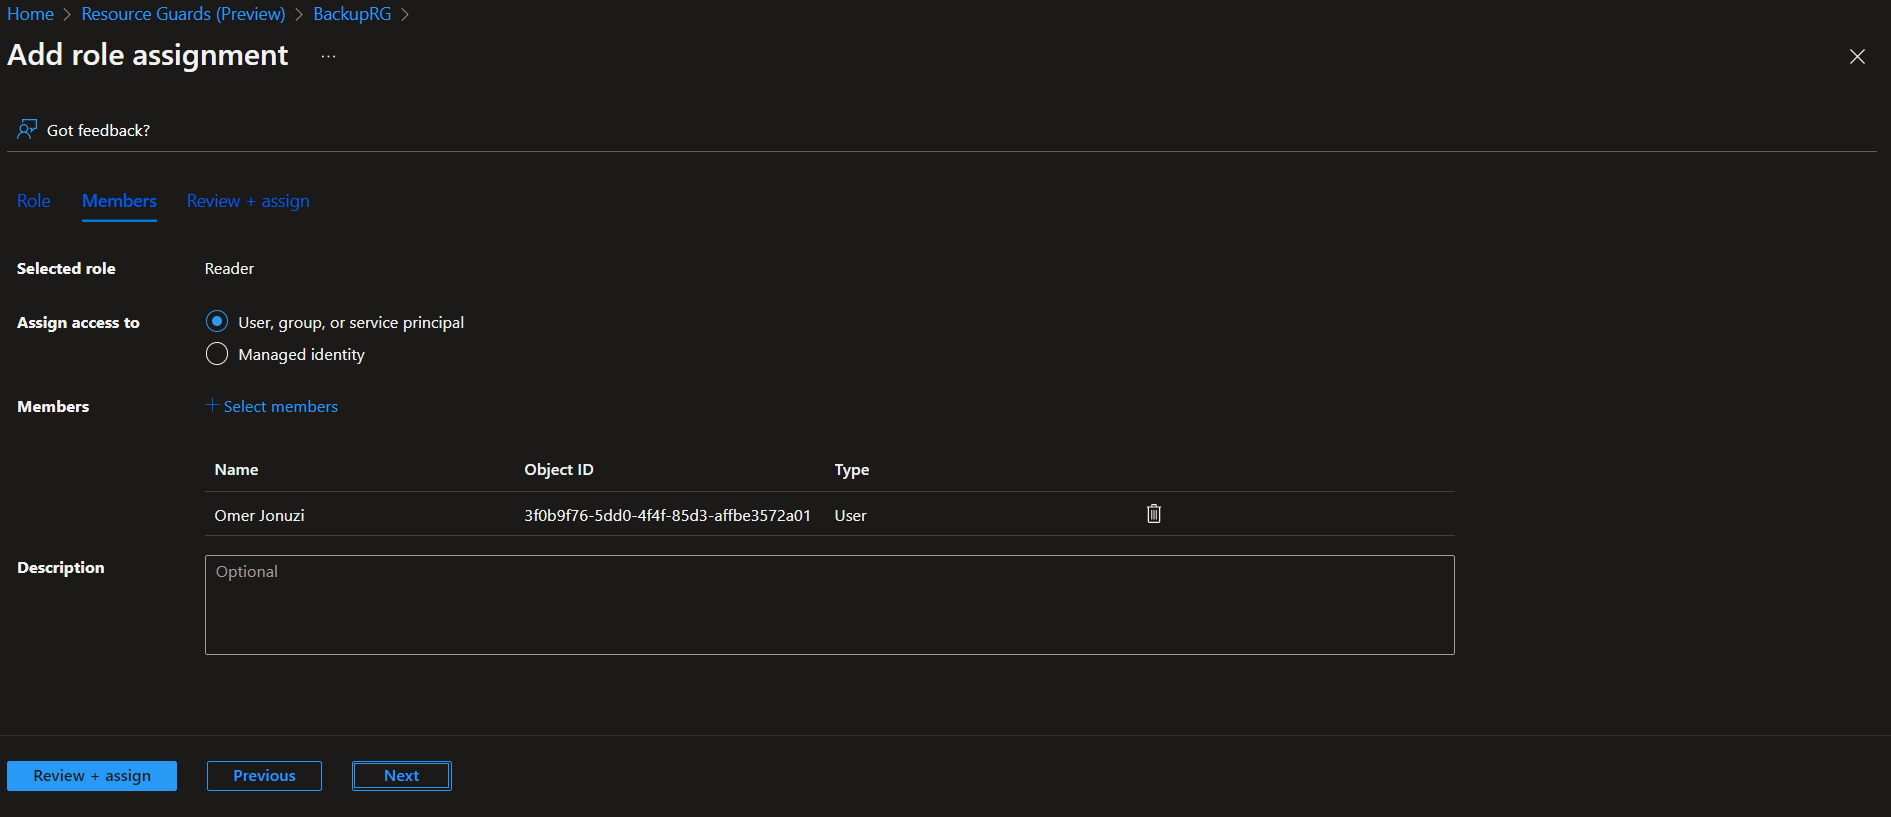
\includegraphics[width=.9\linewidth]{figures/RG-user.PNG}

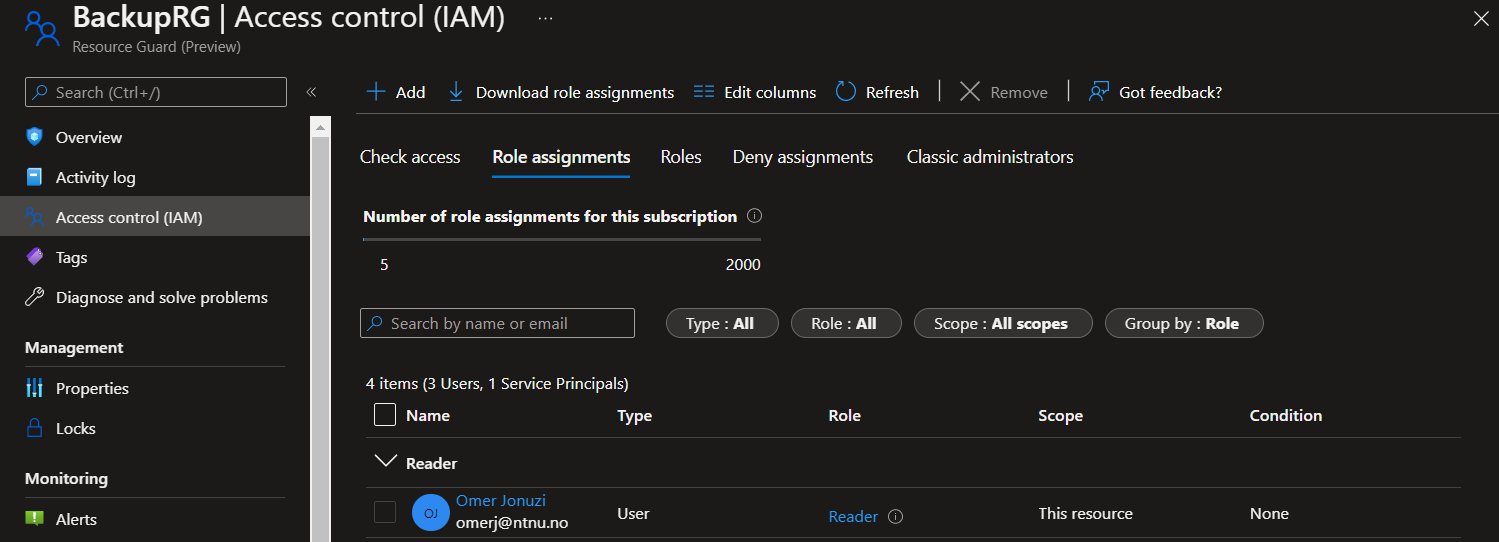
\includegraphics[width=.9\linewidth]{figures/RG-ACblade.PNG}


After the reader role has been granted, the backup administrator can choose to protect any Recovery Service vault with multi-user authorization. To do this they must choose which resource guard to protect it with, which is why the reader role is required. If they do, any protected operation, such as disabling soft-delete or turning MUA off again, should fail as they do not have the necessary permissions on the resource guard. 

\subsection{Applying MUA to vault}
\label{app:chs3e3}
We created a Recovery Services vault, added a resource guard and attempted to disable soft delete.

\paragraph{Create a Recovery Services vault}
\label{sec:org0ba319f}
Since the RSV was deleted in the last experiment,
we made a new one.

Create RSV:
\begin{minted}[breaklines=true,breakanywhere=true]{powershell}
az backup vault create --location $location --name $RSVName --resource-group $RGName
\end{minted}

Output:
\begin{minted}[breaklines=true,breakanywhere=true]{json}
{
  "etag": "W/\"datetime'2022-05-13T13%3A13%3A28.4632743Z'\"",
  "id": "/subscriptions/4b48eb85-91f3-4902-b74b-e84641fb6785/resourceGroups/testRG/providers/Microsoft.RecoveryServices/vaults/myRSV",
  "identity": null,
  "location": "eastus",
  "name": "myRSV",
  "properties": {
    "encryption": null,
    "privateEndpointConnections": null,
    "privateEndpointStateForBackup": "None",
    "privateEndpointStateForSiteRecovery": "None",
    "provisioningState": "Succeeded",
    "upgradeDetails": null
  },
  "resourceGroup": "testRG",
  "sku": {
    "name": "Standard",
    "tier": null
  },
  "systemData": null,
  "tags": null,
  "type": "Microsoft.RecoveryServices/vaults"
}
\end{minted}
\paragraph{Add resource guard}
\label{sec:org4eeccf2}
Press update MUA settings:
\begin{center}
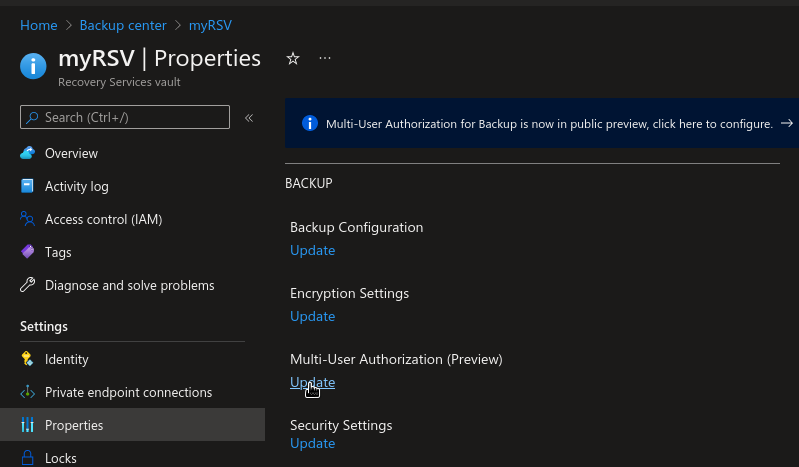
\includegraphics[width=.9\linewidth]{figures/mua/update_rsv_mua.png}
\end{center}

Select resource guard:
\begin{center}
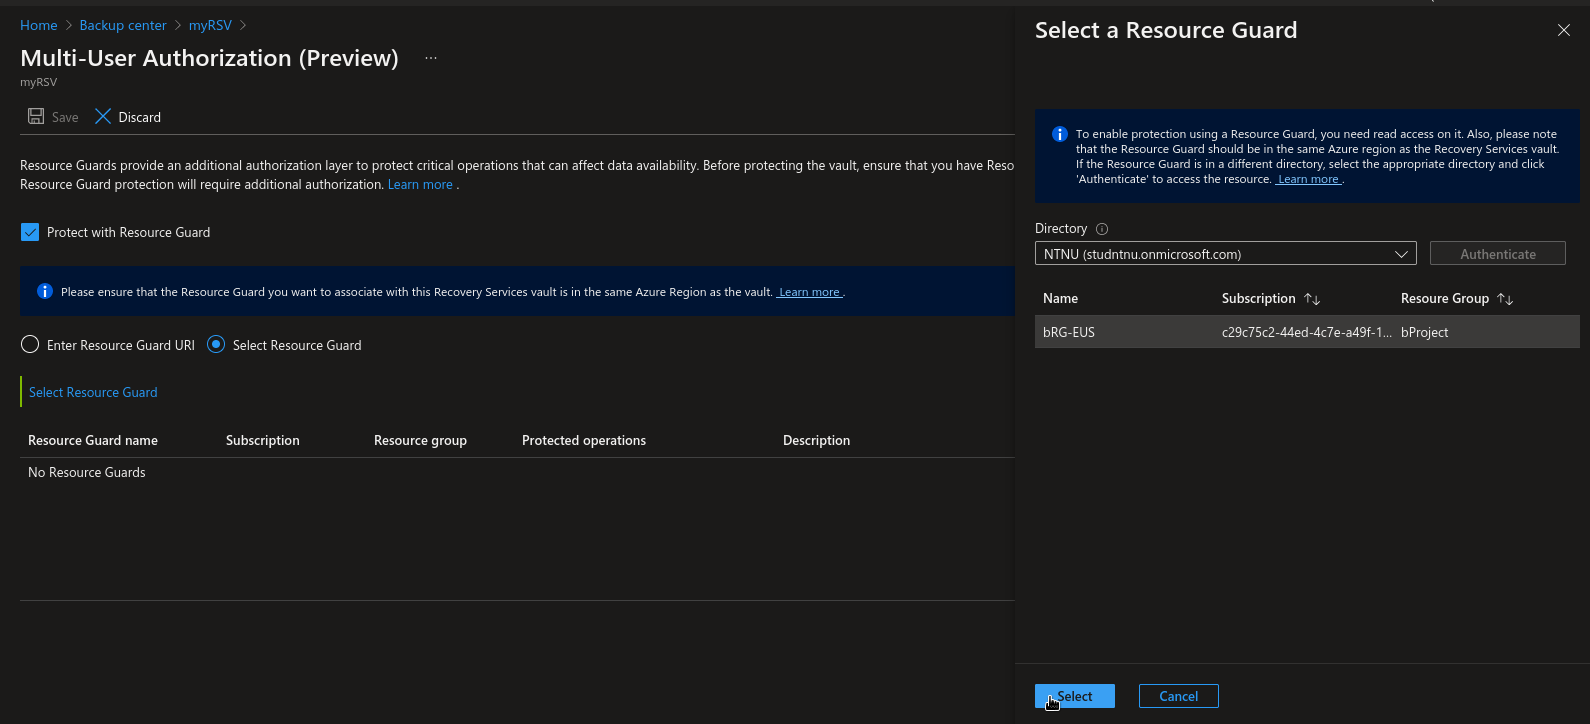
\includegraphics[width=.9\linewidth]{figures/mua/select_resource_guard.png}
\end{center}

Save settings:
\begin{center}
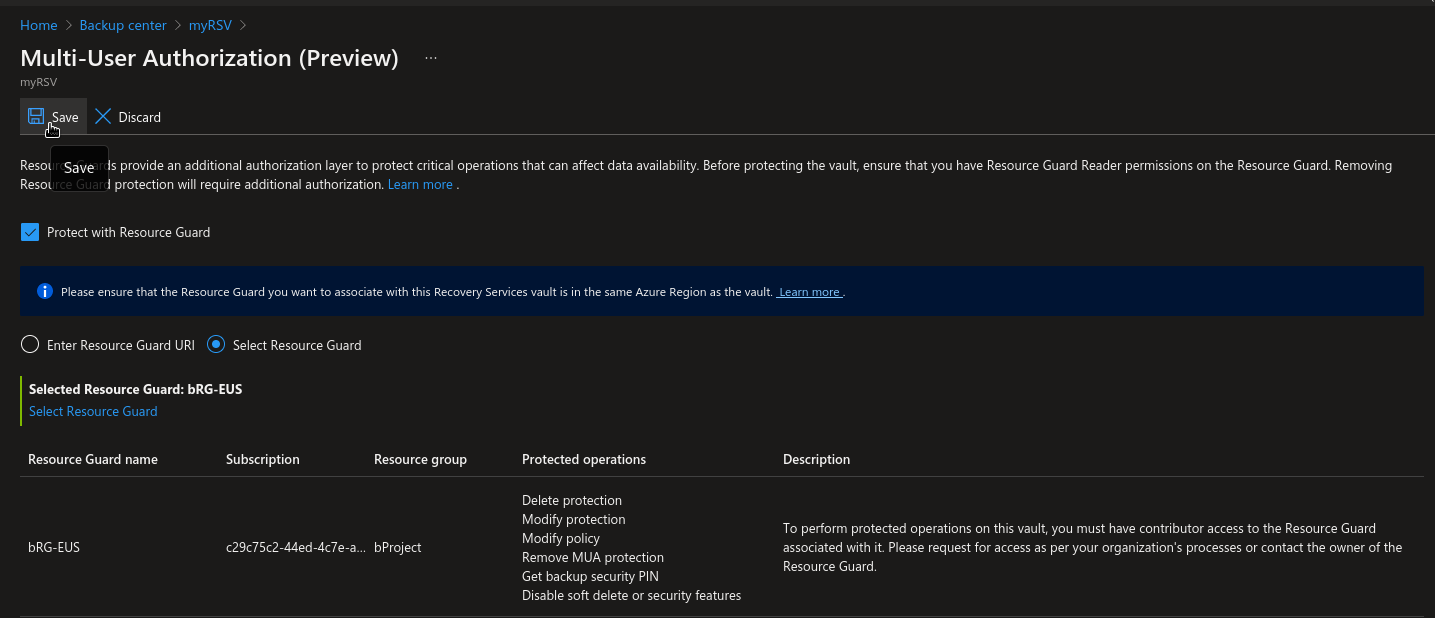
\includegraphics[width=.9\linewidth]{figures/mua/save_mua_settings.png}
\end{center}

\subsection{Testing protected action}
\paragraph{Try to disable soft delete via Azure CLI}
\label{sec:org532e6eb}
An attempt was made at disabling soft delete via the Azure CLI.
The request failed with a generic ``BadRequest'' status code,
presumably because of MUA.

\begin{minted}[breaklines=true,breakanywhere=true]{powershell}
# Get RSV
$RSV = Get-AzRecoveryServicesVault -Name $RSVName -ResourceGroupName $RGName

# Disable soft delete
Set-AzRecoveryServicesVaultProperty -VaultId $RSV.ID -SoftDeleteFeatureState Disable
# Set-AzRecoveryServicesVaultProperty: One or more errors occurred. (Operation returned an invalid status code 'BadRequest')
\end{minted}

\paragraph{Try to disable soft delete via Azure Portal}
\label{sec:orgf58e754}
We attempted to disable soft delete via the Azure Portal.

Disabling soft delete for the vault:
\begin{center}
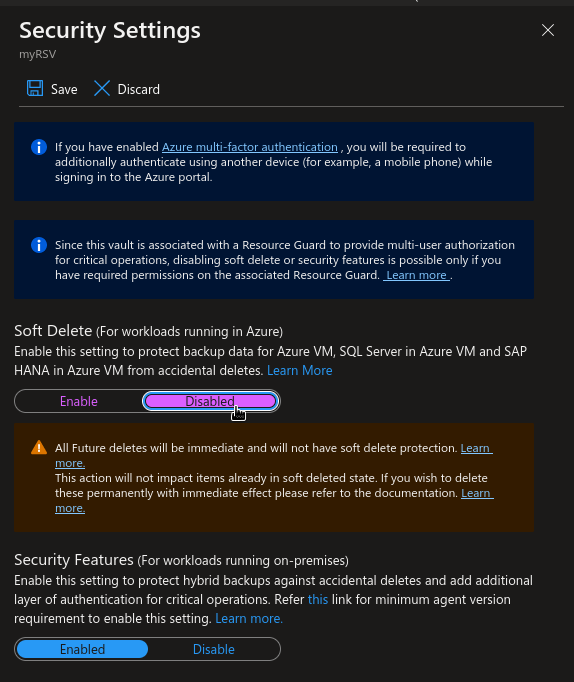
\includegraphics[width=.9\linewidth]{figures/mua/disable_soft_delete.png}
\end{center}

An error appeared in the notifications:
\begin{center}
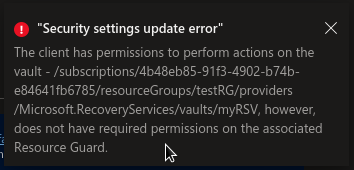
\includegraphics[width=.9\linewidth]{figures/mua/error_mua.png}
\end{center}

\paragraph{Try to run RSV deletion script}
\label{sec:org5bccee7}
The script from [cref] was run once again.
It appears it was able to delete the vault.
We believe this is because the vault is empty.
We attempted a second time with a vault containing backup data.

Output from script:
\begin{minted}[breaklines=true,breakanywhere=true]{text}
Name                                     Account                           SubscriptionName                  Environment                      TenantId
----                                     -------                           ----------------                  -----------                      --------
Azure for Students (4b48eb85-91f3-4902-… MSI@50342                         Azure for Students                AzureCloud                       09a10672-822f-4467-a5ba-5bb3759…

ResourceName      : myRSV
ResourceGroupName : testRG
ResourceNamespace : Microsoft.RecoveryServices
ResouceType       : vaults

Set-AzRecoveryServicesVaultProperty: /home/torstein/delete-rsv.ps1:12
Line |
  12 |  Set-AzRecoveryServicesVaultProperty -Vault $VaultToDelete.ID -SoftDel …
     |  ~~~~~~~~~~~~~~~~~~~~~~~~~~~~~~~~~~~~~~~~~~~~~~~~~~~~~~~~~~~~~~~~~~~~~
     | One or more errors occurred. (Operation returned an invalid status code 'BadRequest')

Soft delete disabled for the vault myRSV
Invoke-RestMethod: /home/torstein/delete-rsv.ps1:30
Line |
  30 |  $response = Invoke-RestMethod -Uri $restUri -Headers $authHeader -Bod …
     |              ~~~~~~~~~~~~~~~~~~~~~~~~~~~~~~~~~~~~~~~~~~~~~~~~~~~~~~~~~
     | {"error":{"code":"InvalidSubscriptionId","message":"The provided subscription identifier 'Azure for Students' is malformed or invalid."}}

Disabled and deleted Azure VM backup items
Disabled and deleted SQL Server backup items
Disabled auto-protection and deleted SQL protectable items
Deleted SQL Servers in Azure VM containers
Disabled and deleted SAP HANA backup items
Deleted SAP HANA in Azure VM containers
Disabled and deleted Azure File Share backups
Unregistered Storage Accounts
Deleted MARS Servers
Deleted MAB Servers
Deleted DPM Servers
Removed Private Endpoints
Number of backup items left in the vault and which need to be deleted: 0 Azure VMs 0 SQL Server Backup Items 0 SQL Server Backup Containers 0 SQL Server Instances 0 SAP HANA backup items 0 SAP HANA Backup Containers 0 Azure File Shares 0 Storage Accounts 0 MARS Servers 0 MAB Servers 0 DPM Servers 0 Private endpoints
Number of ASR items left in the vault and which need to be deleted: 0 ASR protected items 0 ASR policy mappings 0 ASR Fabrics 0 Private endpoints. Warning: This script will only remove the replication configuration from Azure Site Recovery and not from the source. Please cleanup the source manually. Visit https://go.microsoft.com/fwlink/?linkid=2182781 to learn more

Response : Vault has been deleted
\end{minted}

List RSVs:
\begin{minted}[breaklines=true,breakanywhere=true]{powershell}
az backup vault list
\end{minted}

\begin{minted}[breaklines=true,breakanywhere=true]{json}
[
  {
    "etag": "W/\"datetime'2022-05-10T09%3A58%3A14.2637541Z'\"",
    "id": "/subscriptions/4b48eb85-91f3-4902-b74b-e84641fb6785/resourceGroups/perfRG/providers/Microsoft.RecoveryServices/vaults/perfRSV",
    "identity": null,
    "location": "eastus",
    "name": "perfRSV",
    "properties": {
      "encryption": null,
      "privateEndpointConnections": null,
      "privateEndpointStateForBackup": "None",
      "privateEndpointStateForSiteRecovery": "None",
      "provisioningState": "Succeeded",
      "upgradeDetails": null
    },
    "resourceGroup": "perfRG",
    "sku": {
      "name": "Standard",
      "tier": null
    },
    "systemData": null,
    "tags": null,
    "type": "Microsoft.RecoveryServices/vaults"
  }
]
\end{minted}

``myRSV'' is not present in the list.

\paragraph{create new RSV and back up an item}
\label{sec:org3570275}
Create RSV:
\begin{minted}[breaklines=true,breakanywhere=true]{powershell}
az backup vault create --location $location --name $RSVName --resource-group $RGName
\end{minted}

Back up VM:
\begin{minted}[breaklines=true,breakanywhere=true]{powershell}
az backup protection enable-for-vm `
 --resource-group $RGName `
 --vault-name $RSVName `
 --vm $CHName `
 --policy-name $PolicyName
\end{minted}

\paragraph{Add resource guard}
\label{sec:orgc3c211b}
The same procedure was followed as in \hyperref[sec:org4eeccf2]{Add resource guard}.

\paragraph{Try to run RSV deletion script}
\label{sec:orgbb61506}
The script was run once again.
This time, we got a few more errors.
The script still claims that soft delete was disabled,
and that VMs were deleted, but this appears not to be the case.

Output from script:
\begin{minted}[breaklines=true,breakanywhere=true]{text}
Name                                     Account                           SubscriptionName                  Environment                      TenantId
----                                     -------                           ----------------                  -----------                      --------
Azure for Students (4b48eb85-91f3-4902-… MSI@50342                         Azure for Students                AzureCloud                       09a10672-822f-4467-a5ba-5bb3759…

ResourceName      : myRSV
ResourceGroupName : testRG
ResourceNamespace : Microsoft.RecoveryServices
ResouceType       : vaults

Set-AzRecoveryServicesVaultProperty: /home/torstein/delete-rsv.ps1:12
Line |
  12 |  Set-AzRecoveryServicesVaultProperty -Vault $VaultToDelete.ID -SoftDel …
     |  ~~~~~~~~~~~~~~~~~~~~~~~~~~~~~~~~~~~~~~~~~~~~~~~~~~~~~~~~~~~~~~~~~~~~~
     | One or more errors occurred. (Operation returned an invalid status code 'BadRequest')

Soft delete disabled for the vault myRSV
Invoke-RestMethod: /home/torstein/delete-rsv.ps1:30
Line |
  30 |  $response = Invoke-RestMethod -Uri $restUri -Headers $authHeader -Bod …
     |              ~~~~~~~~~~~~~~~~~~~~~~~~~~~~~~~~~~~~~~~~~~~~~~~~~~~~~~~~~
     | {"error":{"code":"InvalidSubscriptionId","message":"The provided subscription identifier 'Azure for Students' is malformed or invalid."}}

Disable-AzRecoveryServicesBackupProtection: /home/torstein/delete-rsv.ps1:49
Line |
  49 |          Disable-AzRecoveryServicesBackupProtection -Item $item -Vault …
     |          ~~~~~~~~~~~~~~~~~~~~~~~~~~~~~~~~~~~~~~~~~~~~~~~~~~~~~~~~~~~~~
     | Unlock privilege access is needed to delete the ResourceGuard proxy

Disabled and deleted Azure VM backup items
Disabled and deleted SQL Server backup items
Disabled auto-protection and deleted SQL protectable items
Deleted SQL Servers in Azure VM containers
Disabled and deleted SAP HANA backup items
Deleted SAP HANA in Azure VM containers
Disabled and deleted Azure File Share backups
Unregistered Storage Accounts
Deleted MARS Servers
Deleted MAB Servers
Deleted DPM Servers
Removed Private Endpoints
Number of backup items left in the vault and which need to be deleted: 1 Azure VMs 0 SQL Server Backup Items 0 SQL Server Backup Containers 0 SQL Server Instances 0 SAP HANA backup items 0 SAP HANA Backup Containers 0 Azure File Shares 0 Storage Accounts 0 MARS Servers 0 MAB Servers 0 DPM Servers 0 Private endpoints
Number of ASR items left in the vault and which need to be deleted: 0 ASR protected items 0 ASR policy mappings 0 ASR Fabrics 0 Private endpoints. Warning: This script will only remove the replication configuration from Azure Site Recovery and not from the source. Please cleanup the source manually. Visit https://go.microsoft.com/fwlink/?linkid=2182781 to learn more
Remove-AzRecoveryServicesVault: /home/torstein/delete-rsv.ps1:204
Line |
 204 |  Remove-AzRecoveryServicesVault -Vault $VaultToDelete
     |  ~~~~~~~~~~~~~~~~~~~~~~~~~~~~~~~~~~~~~~~~~~~~~~~~~~~~
     | Operation failed. ClientRequestId: 9e041d38-0531-4dbb-8db8-63ec5f59f341-2022-05-13 13:41:03Z-P One or more errors occurred. (Recovery Services Vault cannot
     | be deleted as there are existing resources within the vault.  : clickhouseVM. Please ensure all containers have been unregistered from the vault and all
     | private endpoints associated with the vault have been deleted, and retry operation. For more details, see https://aka.ms/AB-AA4ecq5)
\end{minted}

List RSVs:
\begin{minted}[breaklines=true,breakanywhere=true]{powershell}
az backup vault list
\end{minted}

Output:
\begin{minted}[breaklines=true,breakanywhere=true]{json}
[
  {
    "etag": "W/\"datetime'2022-05-10T09%3A58%3A14.2637541Z'\"",
    "id": "/subscriptions/4b48eb85-91f3-4902-b74b-e84641fb6785/resourceGroups/perfRG/providers/Microsoft.RecoveryServices/vaults/perfRSV",
    "identity": null,
    "location": "eastus",
    "name": "perfRSV",
    "properties": {
      "encryption": null,
      "privateEndpointConnections": null,
      "privateEndpointStateForBackup": "None",
      "privateEndpointStateForSiteRecovery": "None",
      "provisioningState": "Succeeded",
      "upgradeDetails": null
    },
    "resourceGroup": "perfRG",
    "sku": {
      "name": "Standard",
      "tier": null
    },
    "systemData": null,
    "tags": null,
    "type": "Microsoft.RecoveryServices/vaults"
  },
  {
    "etag": "W/\"datetime'2022-05-13T13%3A39%3A48.7614362Z'\"",
    "id": "/subscriptions/4b48eb85-91f3-4902-b74b-e84641fb6785/resourceGroups/testRG/providers/Microsoft.RecoveryServices/vaults/myRSV",
    "identity": null,
    "location": "eastus",
    "name": "myRSV",
    "properties": {
      "encryption": null,
      "privateEndpointConnections": null,
      "privateEndpointStateForBackup": "None",
      "privateEndpointStateForSiteRecovery": "None",
      "provisioningState": "Succeeded",
      "upgradeDetails": null
    },
    "resourceGroup": "testRG",
    "sku": {
      "name": "Standard",
      "tier": null
    },
    "systemData": null,
    "tags": null,
    "type": "Microsoft.RecoveryServices/vaults"
  }
]
\end{minted}

The vault (``myRSV'') is still present. In other words the backup administrator was not permitted to delete the vault as long as that involved performing protected actions.

\subsection{Permitting protected actions}
In order to allow for protected actions to be performed on select occasions the reader role will not be sufficient. In order for a backup admin to perform protected actions within a resource guard's scope, they need the contributor-role on that resource guard. In order to to harness the security benefits of just-in-time access and multi user authorization, this can be configured with Azure Active Directory (Azure AD) Privileged Identity Management (PIM). 

The end goal is for the backup admin to be able to raise a request for the contributor role on the resource guard, and temporarily be permitted to perform protected actions. 

In PIM, the security admin must create an eligible assignment for the backup admin as contributor. In short, allowing for the backup admin to request the necessary access. 

In Azure AD privileged identity management we navigate to the resource guard as shown, navigate within it, and click on assignments:

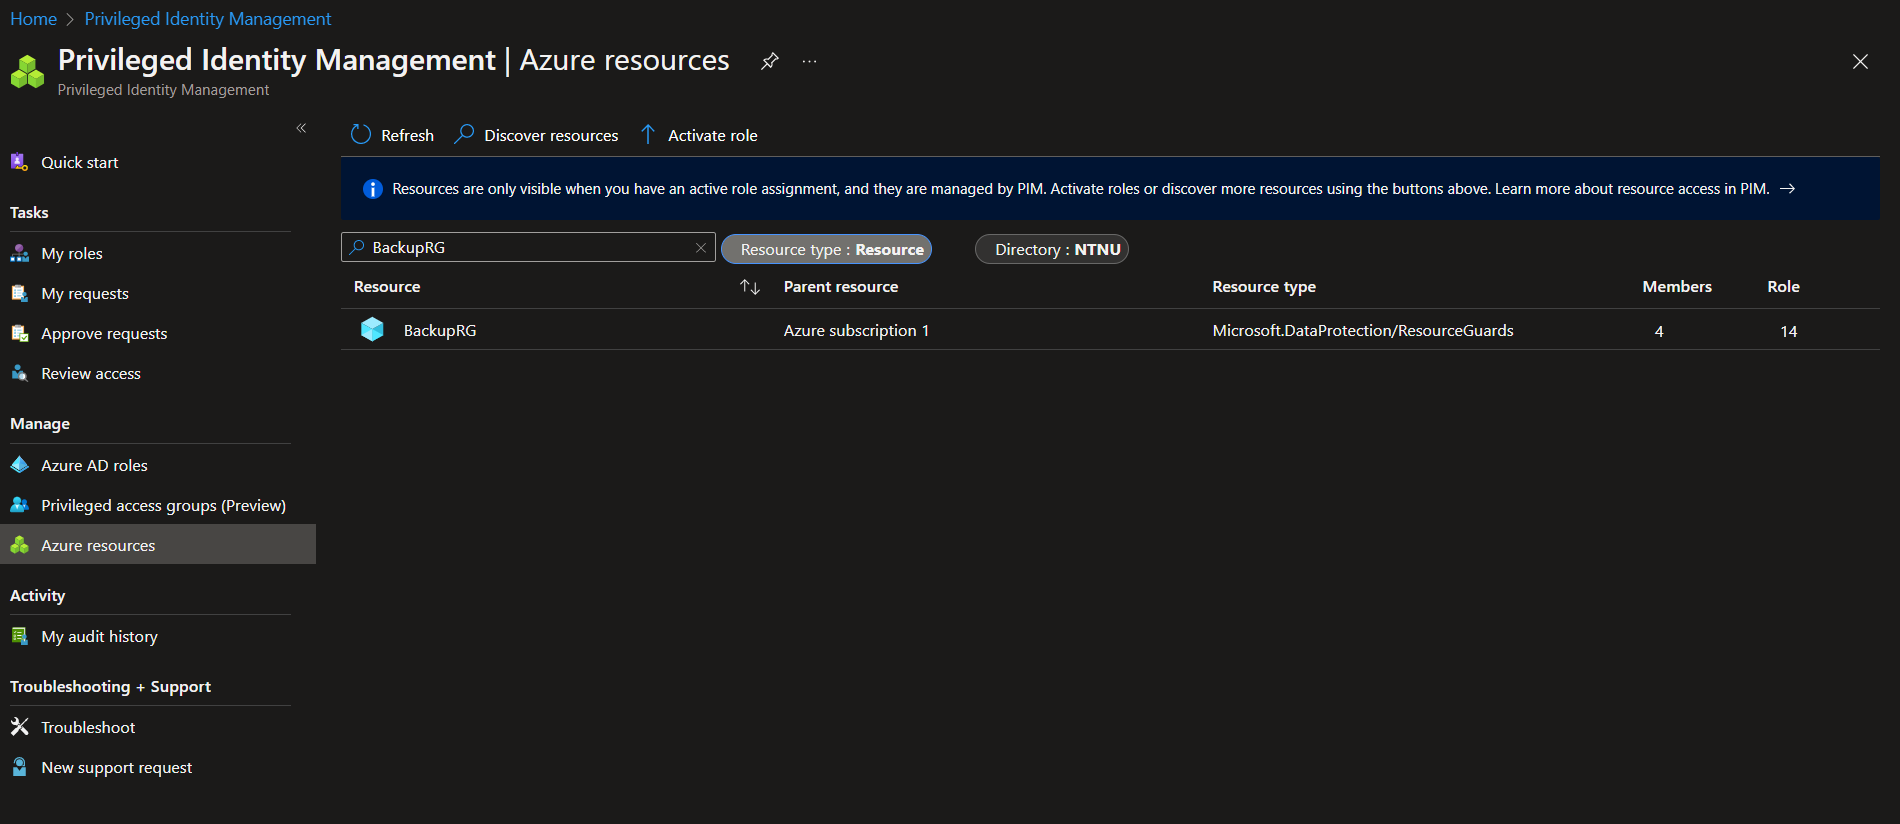
\includegraphics[width=.9\linewidth]{figures/RG-PIM.PNG}

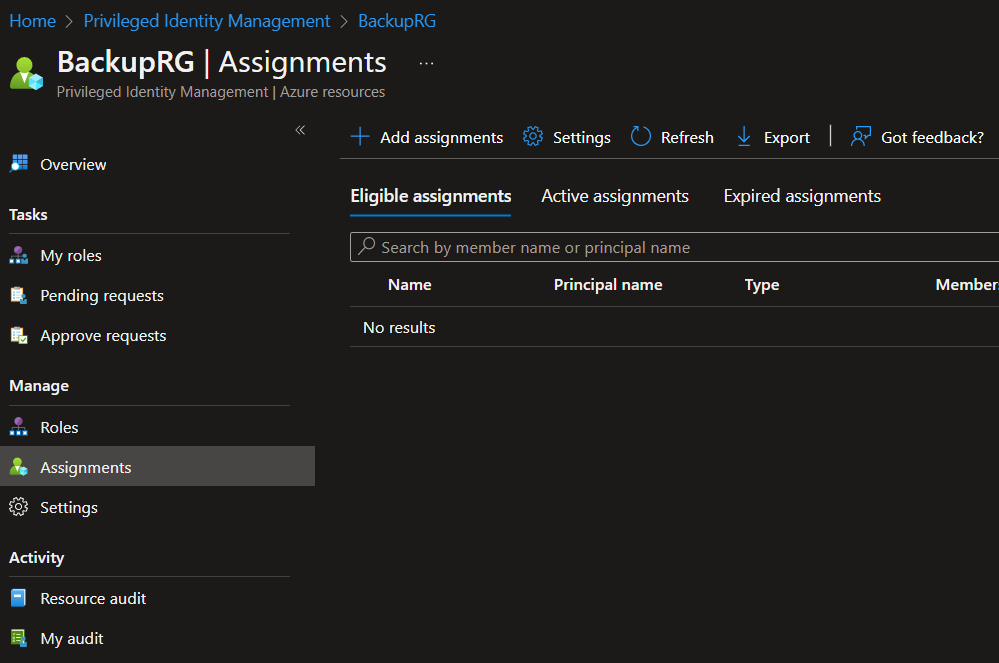
\includegraphics[width=.9\linewidth]{figures/RG-assignments.PNG}

From here we add a new assignment, select the contributor role and our backup admin. THe security admin can choose to grant the assignent for a limitied amount of time, and from here set some settings for maximum duration, and the requirement of a justification before granting the assigned role. By selecting the assignemnt as "elligable", instead of "active", the backup admin must request to have the assigned role activated for them each time they need it. This must then be approved for the amount of time needed until it is automatically revoked. 

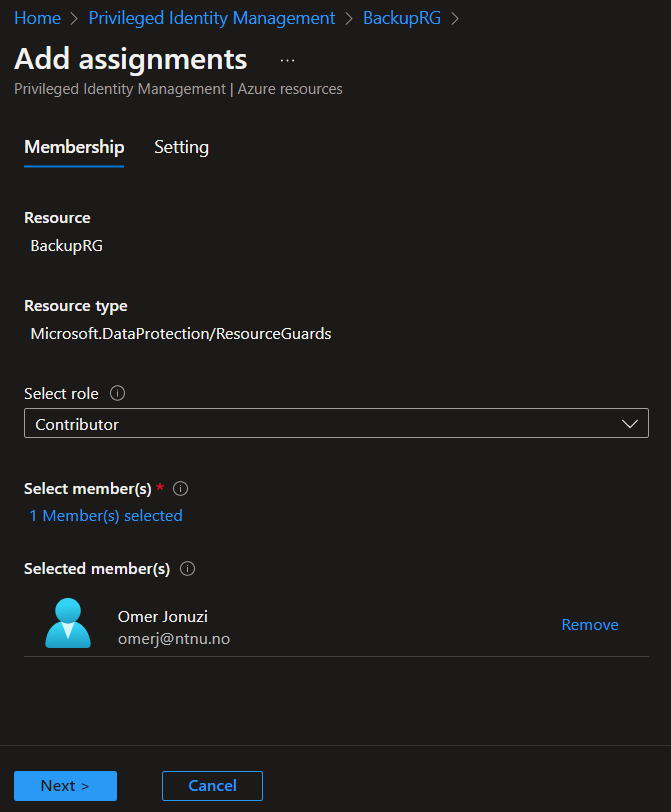
\includegraphics[width=.9\linewidth]{figures/RG-AddAssignment.PNG}

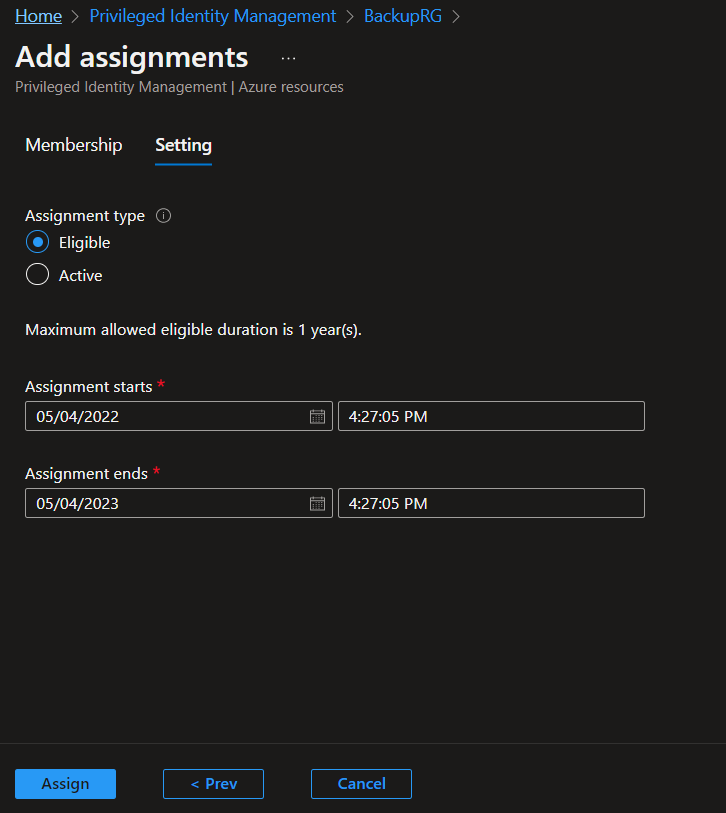
\includegraphics[width=.9\linewidth]{figures/RG-eligible.png}

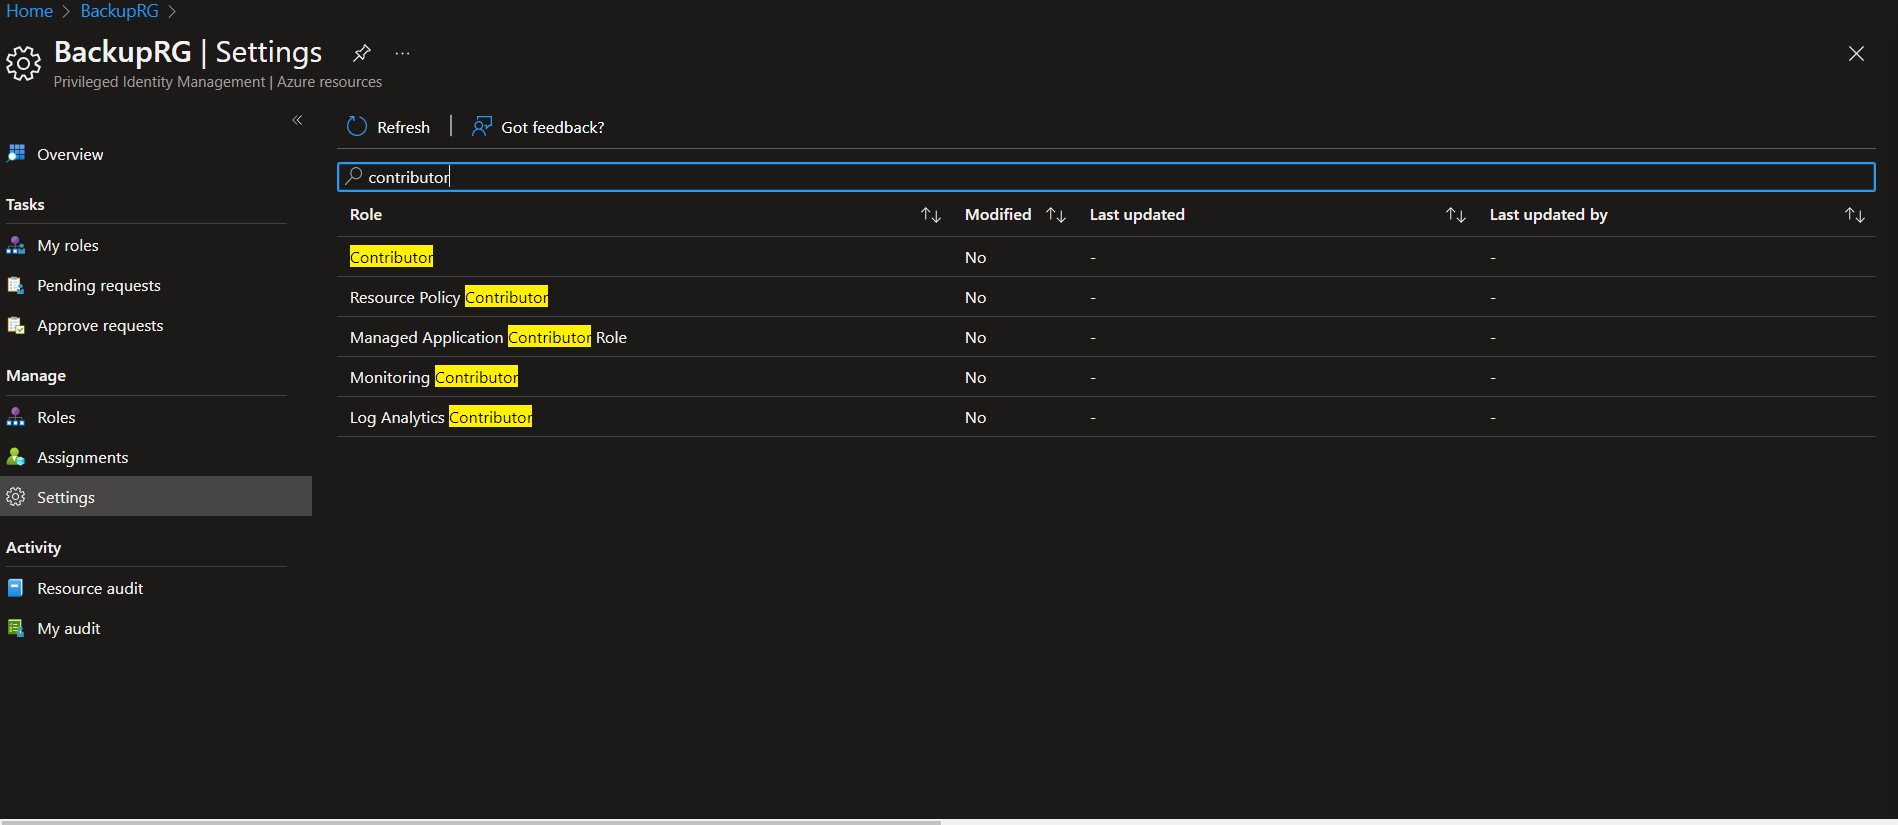
\includegraphics[width=.9\linewidth]{figures/RG-setting.PNG}

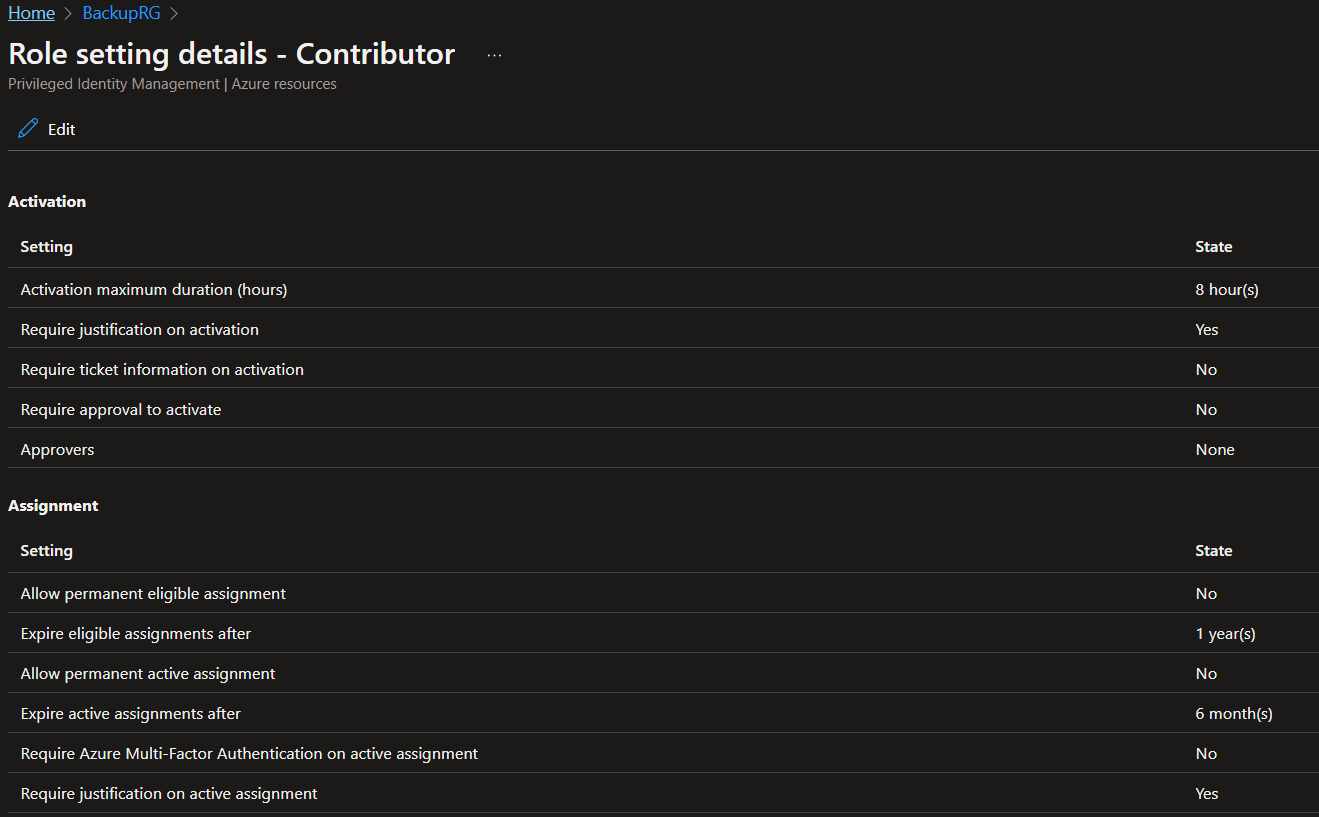
\includegraphics[width=.9\linewidth]{figures/RG-setting-detailts.PNG}

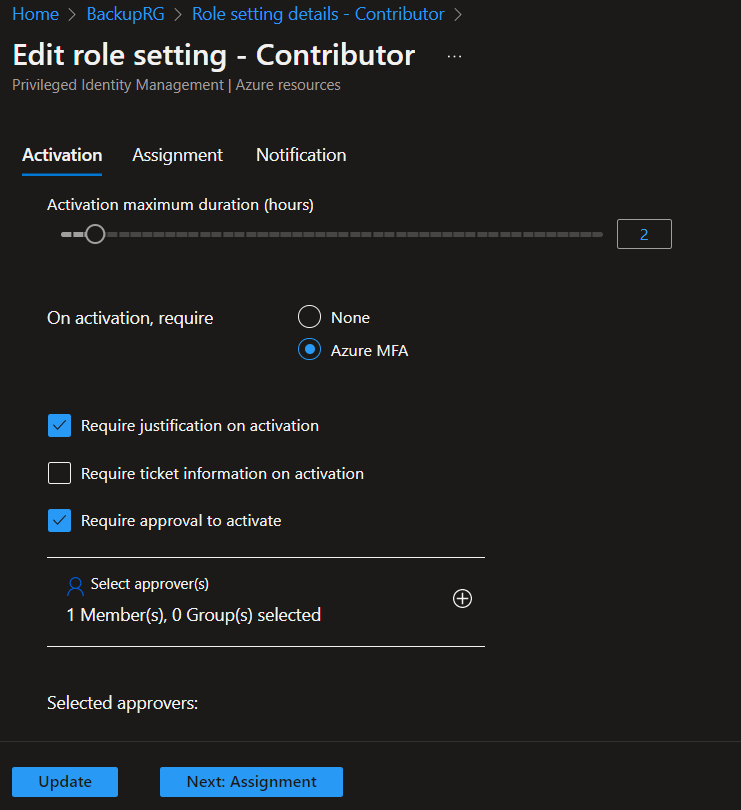
\includegraphics[width=.9\linewidth]{figures/RG-role-setting.PNG}



\paragraph{Request access to contributor role}
\label{sec:orgec87294}
Requesting access to the contributor role:
\begin{center}
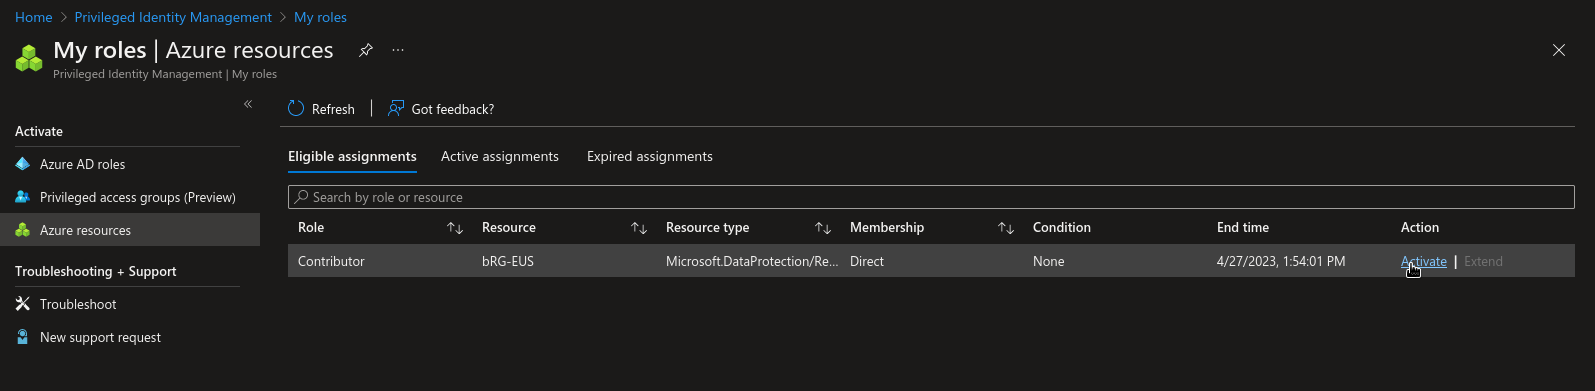
\includegraphics[width=.9\linewidth]{figures/mua/request_role.png}
\end{center}

Sending request:
\begin{center}
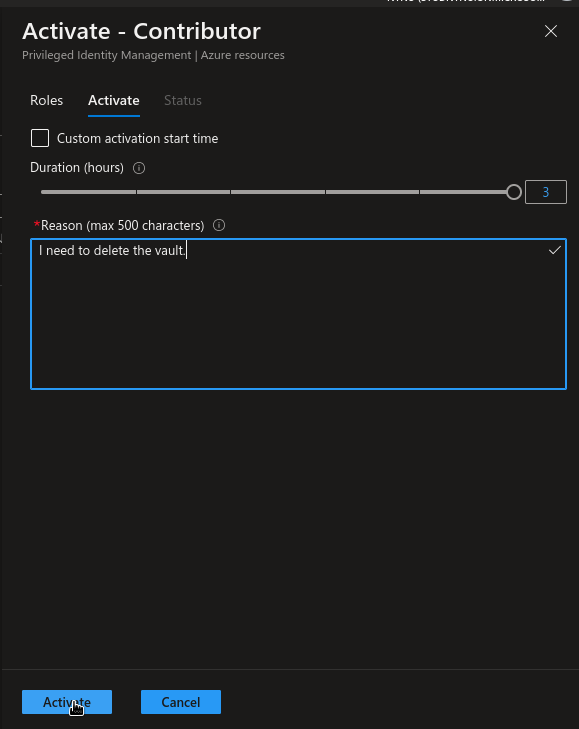
\includegraphics[width=.9\linewidth]{figures/mua/request_mua_role.png}
\end{center}

From the security administrators POV,
A request has been recieived in the PIM-service:

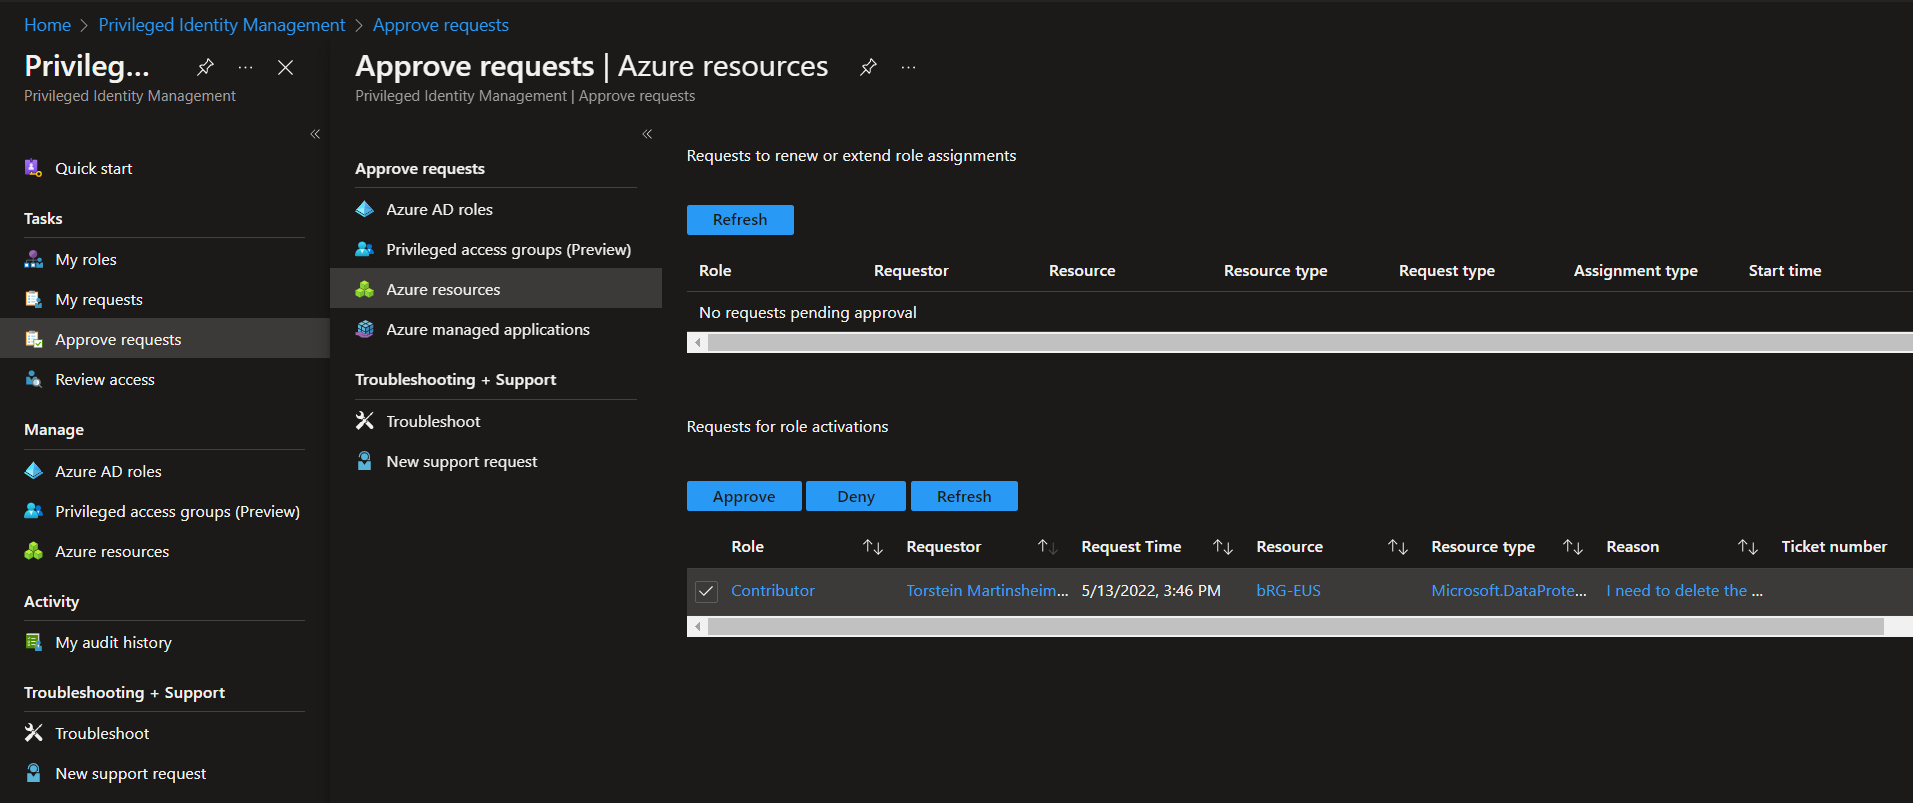
\includegraphics[width=.9\linewidth]{figures/mua/Request.PNG}

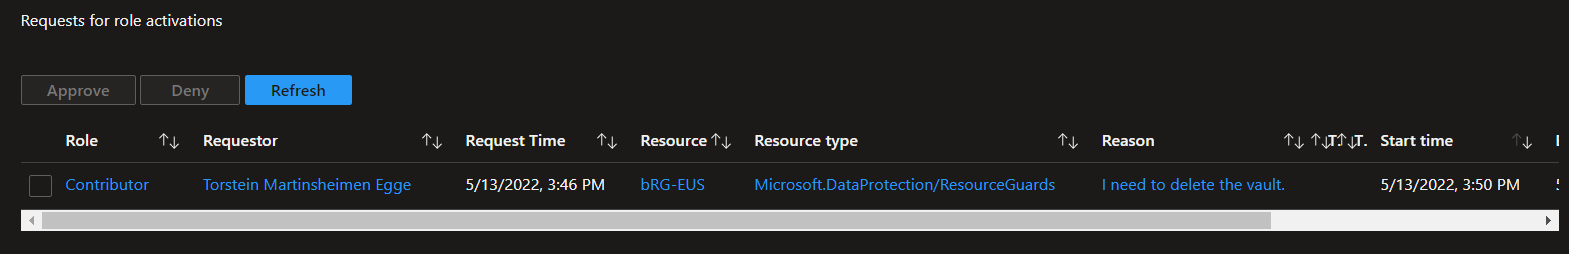
\includegraphics[width=.9\linewidth]{figures/mua/Capture.PNG}

The request is activated by security admin as shown:

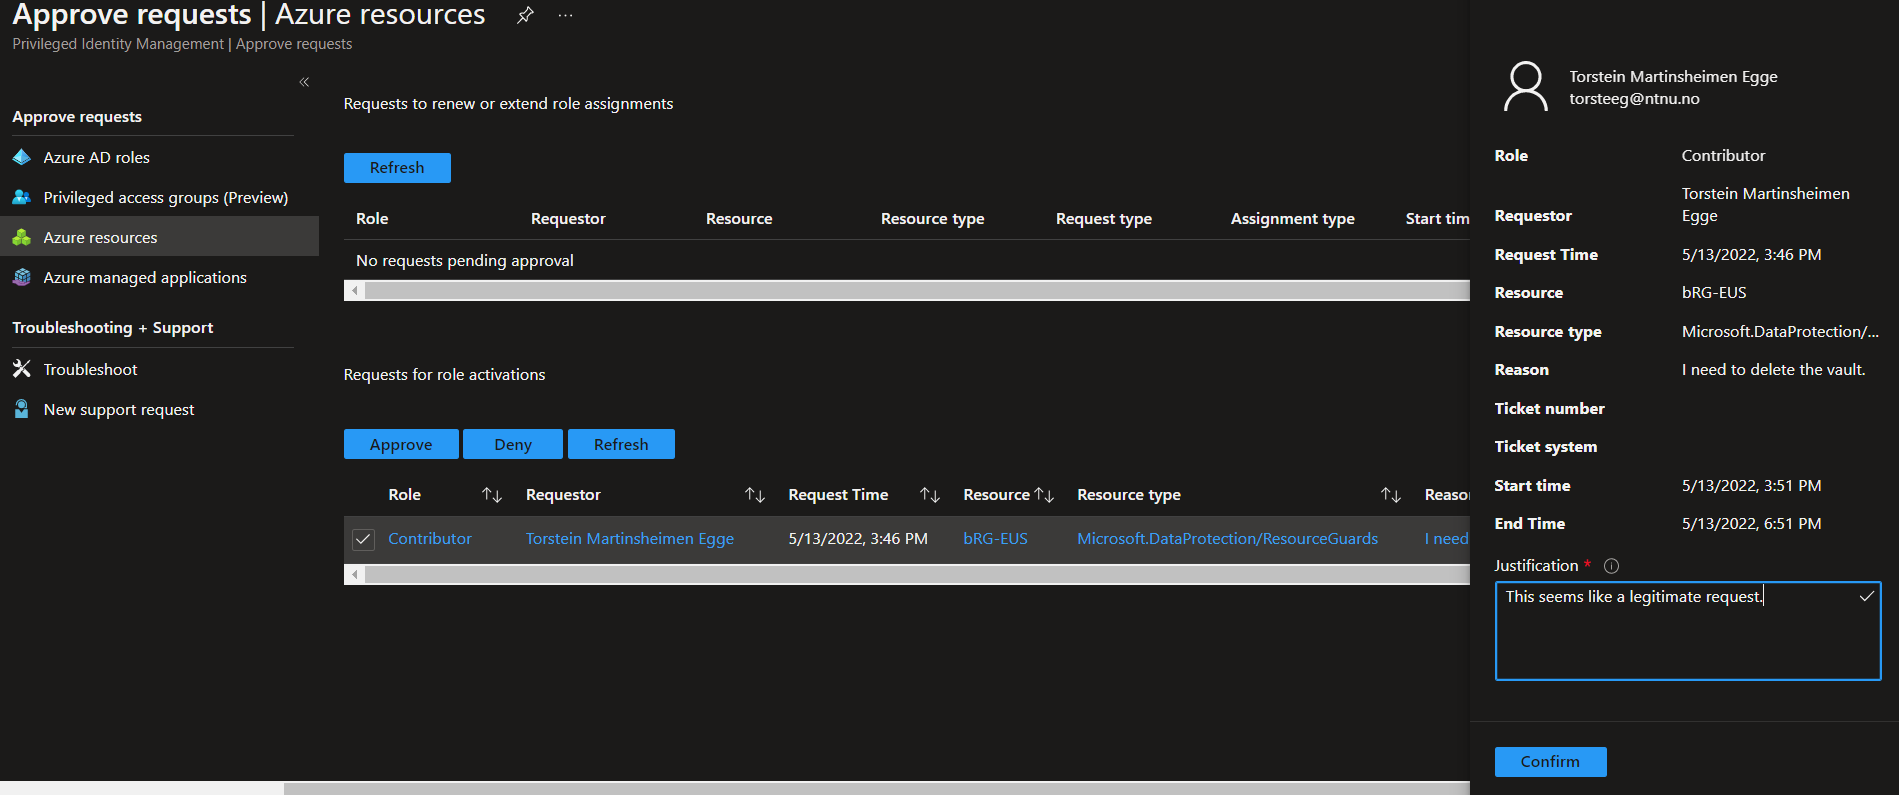
\includegraphics[width=.9\linewidth]{figures/mua/approve.PNG}


An email was received by the backup admin when the request was accepted:
\begin{center}
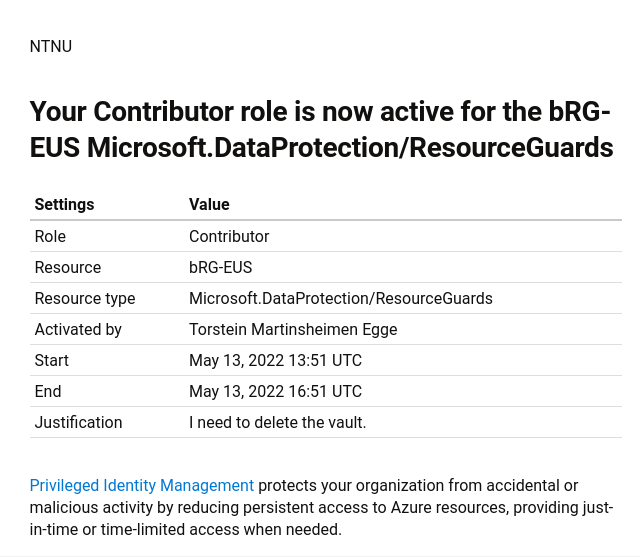
\includegraphics[width=.9\linewidth]{figures/mua/role_active_email.png}
\end{center}

\paragraph{Try to disable soft delete}
\label{sec:org6ff9cf1}
Soft delete was successfully disabled for the vault:
\begin{center}
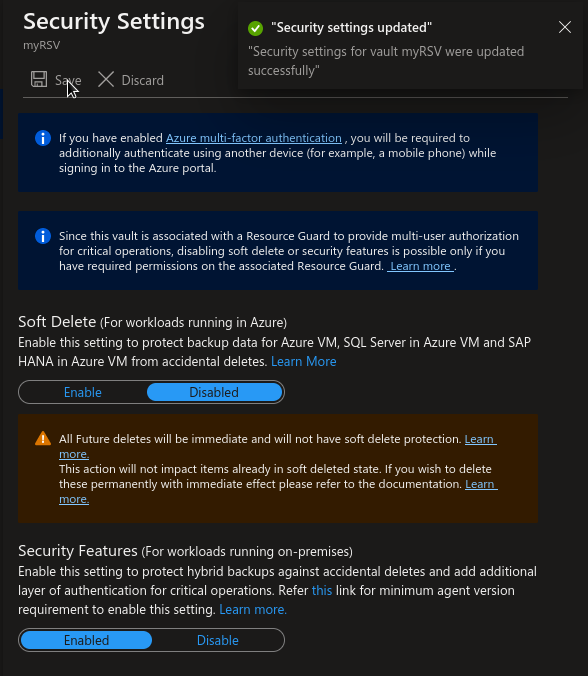
\includegraphics[width=.9\linewidth]{figures/mua/soft_delete_disabled.png}
\end{center}
